The first word embedding framework presented here was introduced by \citet{mikolov2013efficient} and has been proven to outperform the previously best performing techniques regarding semantic and syntactic word relationship tests in the paper.

The intuition behind Word2Vec word embeddings is that it trains a neural network on a binary prediction task and afterwards returns the weights of the neural network trained on this task which constitute the embeddings for the words \citep{embedding2020pilehvar}.

This prediction task depends on the used architecture presented in \citet{mikolov2013efficient}, the continuous bag-of-words (CBOW) and skipgram (SG).

The CBOW architecture is implemented by the task of predicting a target word given a certain number of context words that surround it. The amount of context words used is defined by the window size which sets the number of preceding and subsequent words to consider \citep{rehurek2022w2v}.

In figure \ref{fig:w2v} a) a target word $w_i$ shall be predicted using a window size of 2. Therefore the input for this predictive task are the two preceding words $w_{i-2}, w_{i-1}$ and the two subsequent words $w_{i+1},w_{i+2}$.
These four words are combined by being averaged or summed up and fed into the projection layer. By combining them the order of the context words gets lost which is the reason \citet{mikolov2013efficient} has coined this architecture a bag-of-words model. Afterwards a log-linear classifier tries to predict the target word.

\begin{figure}
    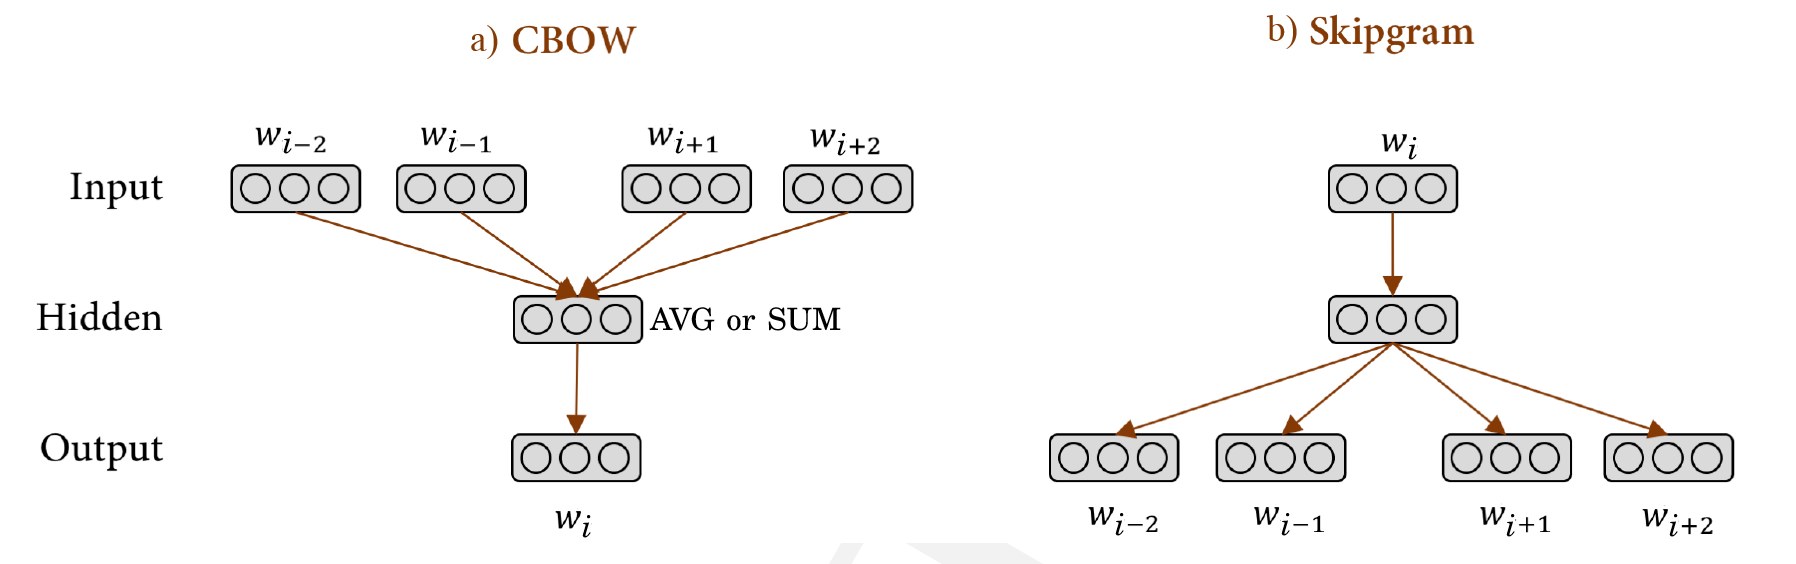
\includegraphics[width=\linewidth]{Pictures/Pilehvar_20_w2v.png}
    \caption{Adapted and modified from \citet{embedding2020pilehvar}: Visualization of the two prediction tasks present in the Word2Vec framework with a window size of 2. \newline 
    a) CBOW: $w_i$ constitutes the target word which shall be predicted using the two preceding and subsequent words. \newline
    b) Skipgram: $w_i$ constitutes the input (middle word) which shall be used to predict the two preceding and subsequent words.}
    \label{fig:w2v}
\end{figure}

Figure \ref{fig:w2v} b) visualizes the second architecture, the skipgram approach. Here $w_i$ serves as the input to the model, is fed to the projection layer and a log-linear classifier tries to predict the words in the context \citep{mikolov2013efficient}, in this case $w_{i-2}, w_{i-1},w_{i+1},w_{i+2}$. Therefore one instance for the training process is the tuple of the middle word $w_i$ and either one of its context words as a positive example or a word that does not appear in its context as a negative example. 

Since such tuples could be created for each combination of the vocabulary and this would result in innumerous cases, the process called negative sampling chooses a limited number of combinations of the middle word and words that did not appear in its context \citep{karimi2021sampling}.
Additionally since the relatedness of words declines once you move further away from a certain word, combinations of the middle word and words in its context, but relatively far away, are sampled less frequently \citep{mikolov2013efficient}.

For both architectures the log-linear classifier then has to distinguish the positive cases in which the samples are made up of words that belong to the same context and the negative samples \citep{jurafsky2021}.

Once the training process for the prediction task is finished, it is no longer relevant since the word embeddings are obtained by extracting the weight matrix of the projection layer \citep{mikolov2013efficient}.

As shown by \citet{mikolov2013efficient} these techniques result in word embeddings that provide valuable information on the syntactic and semantic relatedness of words when trained on very huge datasets.

The fact that for training the word embeddings the running text itself provides the input and correct output like a supervised task is called self-supervision and provides, as \citet{jurafsky2021} put it, a 'revolutionary intuition' for effective word embedding training.




